\chapter{Theoretical Background on Thermal Radiation}
%\addcontentsline{toc}{chapter}{Theoretical background on thermal radiation}

This chapter describes fundamental principles and concepts of EM radiation called \textit{thermal radiation}. Every object with temperature above 0 K emits thermal radiation. The amount of thermal radiation as a function of wavelength depends on object's temperature and its surface as is described in following text.

\subsubsection*{Black body}
The concept of black body is very well described in the work of Howell \cite{H11}, where black body is defined as perfect absorber for all incident radiation. Apart of perfect absorber, the black body is perfect emitter as well. Thus black body absorbs and reemits all energy incident upon it. Black body does not exist in nature but its concept is used for determination of real object's surface property called emissivity, which will be defined in following text. 

\subsubsection*{Planck's law}
Concerning black body at thermal equilibrium, the amount and spectral distribution of emitted energy is described by Planck’s law \cite{P00}:
$$B(T,\lambda) = \frac{2hc^2}{\lambda^5}\frac{1}{e^{\frac{hc}{\lambda k T}}-1},$$
where $B(T,\lambda)$ is spectral radiance ($\SI{}{\watt}\,\SI{}{\meter}^{-2}\,\SI{}{\micro\meter}^{-1}\,\SI{}{\steradian}^{-1}$) of black body at temperature $T$ ($\SI{}{\kelvin}$) and wavelength $\lambda$ ($\SI{}{\micro\meter}$); $k$ is Boltzmann constant ($1.3806488\cdot10^{-23}\,\SI{}{\joule}\,\SI{}{\kelvin}^{-1}$), $h$ is Planck constant ($6.62606957\cdot10^{-34}\,\SI{}{\joule}\,\SI{}{\second}$) and $c$ is speed of light ($299792458\,\SI{}{\meter}\,\SI{}{\second}^{-1}$). Example of the black body radiation at three different temperatures, as described by Planck's law, is depicted in figure \ref{fig:BBradiation}.

\subsubsection*{Emissivity}
The emissivity is defined as ratio of radiance of real surface to that of black body at the same temperature:
$$ \varepsilon(T,\lambda) = \frac{L(T,\lambda)}{B(T,\lambda)},$$
where $\varepsilon(T,\lambda)$ is spectral emissivity and $L(T,\lambda)$ is real surface spectral radiance. The emissivity can be understood as real surface emission effectiveness in comparison with radiation emitted by a black body of the same temperature in the same wavelength. Let us note that emissivity depends on the viewing angle apart temperature and wavelength, as is defined in Hollow \cite{H11}. In remote sensing an observed objects are of the temperature within 270 – 330 K and the observation angle is close to nadir (usually maximum off-nadir angle is less than 30$^\circ$), which causes negligible changes in spectral emissivity of most~of the natural surfaces. Thus, it can be further assumed that emissivity depends just on~wavelength. 

Quartz was chosen to demonstrate the principles of radiation of real object's surfaces. Its spectral emissivity was taken from ASTER spectral library \cite{BH09} and it is shown in the figure \ref{fig:QuartzEmissivity}. Quartz heated to the temperature $T$ has spectral radiance $L(T,\lambda) = \varepsilon(\lambda) B(T,\lambda)$ as is illustrated in figure \ref{fig:QuartzRadiance}. 

\begin{figure}[htb]
	\centering
	\vspace{1em}
	\begin{subfigure}[t]{.3\linewidth}
		\centering
		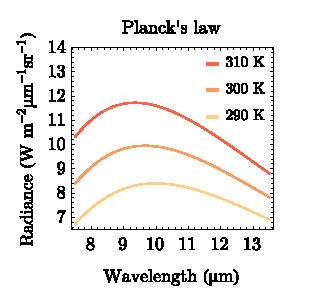
\includegraphics[scale=1]{pics/Chapter_01/PlancksLaw.eps}
		\vspace{-0.1cm}
		\caption{Radiation of black body described by Planck's law}
		\label{fig:BBradiation}
	\end{subfigure}
	\hspace{1em}
	\begin{subfigure}[t]{.3\linewidth}
		\centering
		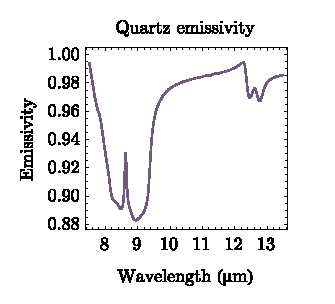
\includegraphics[scale=1]{pics/Chapter_01/QuartzSpectrum.eps}
		\vspace{-0.1cm}
		\caption{Quartz spectral emissivity}
		\label{fig:QuartzEmissivity}
	\end{subfigure}
	\hspace{1em}
	\begin{subfigure}[t]{.3\linewidth}
		\centering
		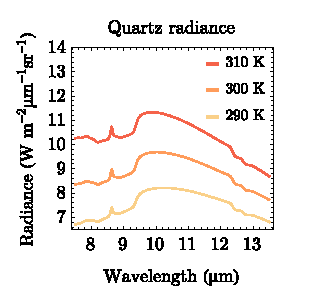
\includegraphics[scale=1]{pics/Chapter_01/QuartzRadiance.eps}
		\vspace{-0.1cm}
		\caption{Radiance of quartz}
		\label{fig:QuartzRadiance}
	\end{subfigure}
	\vspace{1.5 em}
	\caption{Principles of radiation of real surfaces.}
\end{figure}


\subsubsection*{Wien's displacement law}
The peak of black body radiation at wavelength $\lambda_{max}$ is described by Wien's displacement law \cite{H11}:
$$ \lambda_{max} = \frac{b}{T},$$
where $b$ is Wien's displacement constant ($2.8977721\,\SI{}{m}\,\SI{}{K}$). As was mentioned before, the temperature of the most of the natural and artificial surfaces observed by airborne remote sensing ranges in 270 – 330 K. According to the Wien's displacement law, the peak of emitted radiation varies roughly from $8.8\,\SI{}{\micro\meter}$ to $10.7\,\SI{}{\micro\meter}$. This range is in coincidence with the atmospheric window situated between $8\,\SI{}{\micro\meter}$ to $13\,\SI{}{\micro\meter}$. The atmospheric transmittance in this atmospheric window is very high and thus it is relevant for acquisition of remotely sensed thermal data.

\subsubsection*{Kirchhoff's law of thermal radiation}
Emitting and absorbing properties of an object at local thermodynamic equilibrium surrounded by isothermal environment are tied up by Kirchhoff's law of thermal radiation \cite{K60}. It states that object's surface absorptivity $\alpha(\lambda)$ at a given wavelength equals to object surface emissivity $\varepsilon(\lambda)$ at the same wavelength:
$$ \alpha(\lambda) = \varepsilon(\lambda). $$
Energy conservation implies that energy incident to the object surface can be reflected, transmitted or absorbed. Considering the fractions of incident energy the following equation holds:
$$ 1 = \rho(\lambda) + \tau(\lambda) + \alpha(\lambda), $$
where $\rho(\lambda)$ is objects surface spectral reflectivity, $\tau(\lambda)$ is object surface spectral transmissivity and $\alpha(\lambda)$ is object surface spectral absorptivity. Applying Kirchhoff's law to opaque material ($\tau(\lambda) = 0$) results in following equation:
$$ 1 = \rho(\lambda) + \varepsilon(\lambda) \quad \Rightarrow \quad \rho(\lambda) = 1 - \varepsilon(\lambda).$$

All mentioned principles in this section will be further used in explanation of properties of airborne thermal hyperspectral data and its processing.